\section{Datasets}\label{datasets}

In this section we describe the datasets in more detail. The time gap between two events $\DeltaTime^*_\IndexEvent = \Timestamp_\IndexEvent - \Timestamp_{\IndexEvent-1}$ is first log-transformed before applying min-max normalization: $\hat{\DeltaTime_\IndexEvent}^* = \frac{\DeltaTime_\IndexEvent' - \min(\DeltaTime_\IndexEvent^{*'})}{(\max(\DeltaTime_\IndexEvent^{*'}) - \min(\DeltaTime_\IndexEvent^{*'})}$ with $\DeltaTime_\IndexEvent^{*'} = \log(\DeltaTime_\IndexEvent^* + \epsilon)$, $\epsilon > 0$.

\paragraph{3-G.} We use $\NbClasses=3$ and draw from a normal distribution  $P(\DeltaTime | \IndexClass_\IndexEvent) = \mathcal{N}(i + 1, 1.)$. This dataset tries to imitate the setting from Fig.\ \ref{fig:car_categorical} as explained in \ref{sec:introduction_010}. We generate 1000 events. Probability density is shown in figure \ref{fig:k-gaussians-density}. Models that are not taking time into account cannot solve this problem. Below is the code. We create the \textbf{Multi-G} dataset similarly.\vfill

\begin{figure}[H]
\centering
    \begin{subfigure}{.45\textwidth}
        \centering
    	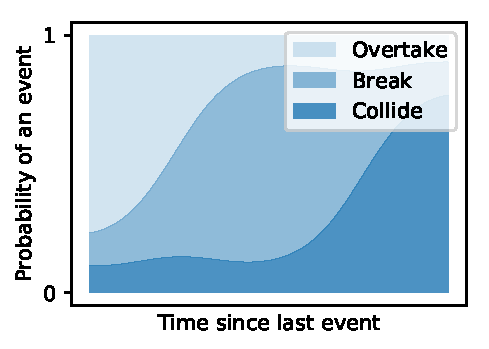
\includegraphics[width=.8\linewidth]{sections/010_neurips2019/paper/images/categorical_evolution.pdf}
        \caption{Car example explained in section \ref{sec:introduction_010} where probabilities of events to occur change over time}
    \label{fig:car_categorical}
    \end{subfigure}%
    \hspace*{10.mm}
    \begin{subfigure}{.45\textwidth}
        \centering
   		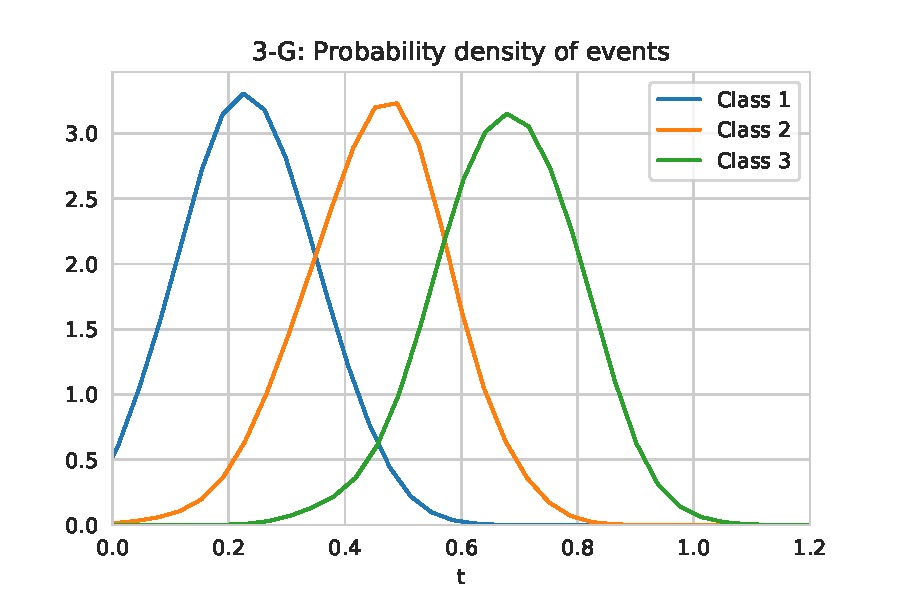
\includegraphics[width=.8 \linewidth]{sections/010_neurips2019/paper/images/k-gaussians-density.pdf}
		\caption{Probability density of events in K-Gaussians dataset. We can see that classes are independent of history.}\label{fig:k-gaussians-density}
    \end{subfigure}
\end{figure}

\begin{minipage}{\linewidth}
\begin{verbatim}
def generate():
    data = np.zeros((1000, 2))
    for i in range(1000):
        i_class = np.random.choice(3, 1)[0]
        time = np.random.normal(i_class + 1, 1.)
        while time <= 0:
            time = np.random.normal(i_class + 1, 1.)
        data[i, 0] = i_class
        data[i, 1] = time
    return data
\end{verbatim}
\end{minipage}

\paragraph{Car Indicators.}
A sequence contains signals from a single car during one ride. We remove signals that are perfectly correlated giving 6 unique classes in the end. Top 3 classes make up 33\%, 32\%, and 16\% of a total respectively. From figure \ref{fig:car-indicators-density} we can see that the setting is again asynchronous.
\begin{figure}[H]
    \centering
    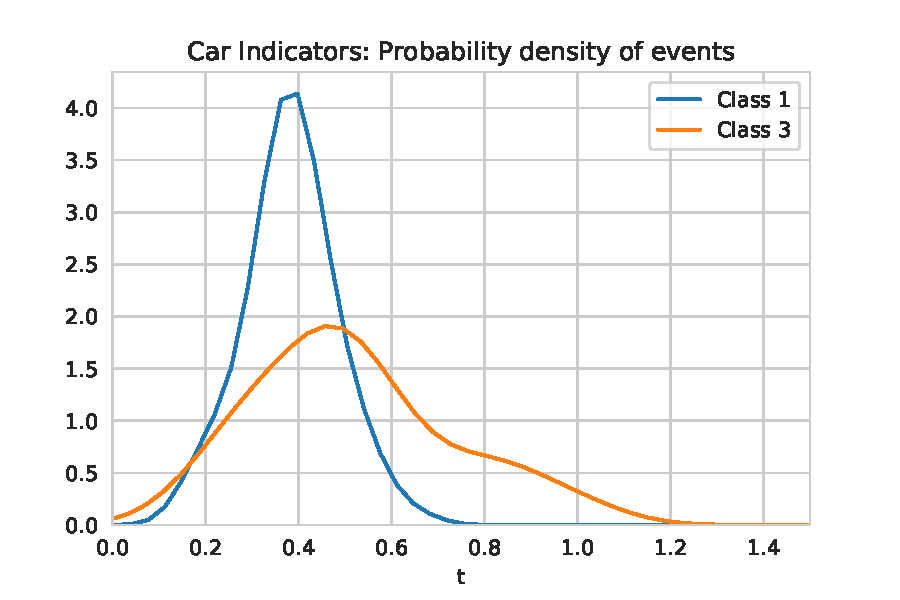
\includegraphics[width=0.35 \linewidth]{sections/010_neurips2019/paper/images/car-indicators-density.pdf}
    \caption{Probability density of events in Car Indicators dataset for 2 selected classes. Time is log-transformed.}\label{fig:car-indicators-density}
\end{figure}

\paragraph{Graph.}

We generate graph $G$ with $10$ nodes and $48$ edges between them. We assign variables $\mu$ and $\sigma$ to each transition (edge) between events (nodes). The time it takes to make a transition between nodes $i$ and $j$ is drawn from normal distribution $\mathcal{N}(\mu_{ij}, \sigma^2_{ij})$. By performing a random walk on the graph we create $10$ thousand events. This dataset is similar to K-Gaussians with the difference that a model needs to learn the relationship between events together with the time dependency. Parts of the trace are shown in figure \ref{fig:random-graph-trace}.
\begin{figure}[H]
    \centering
    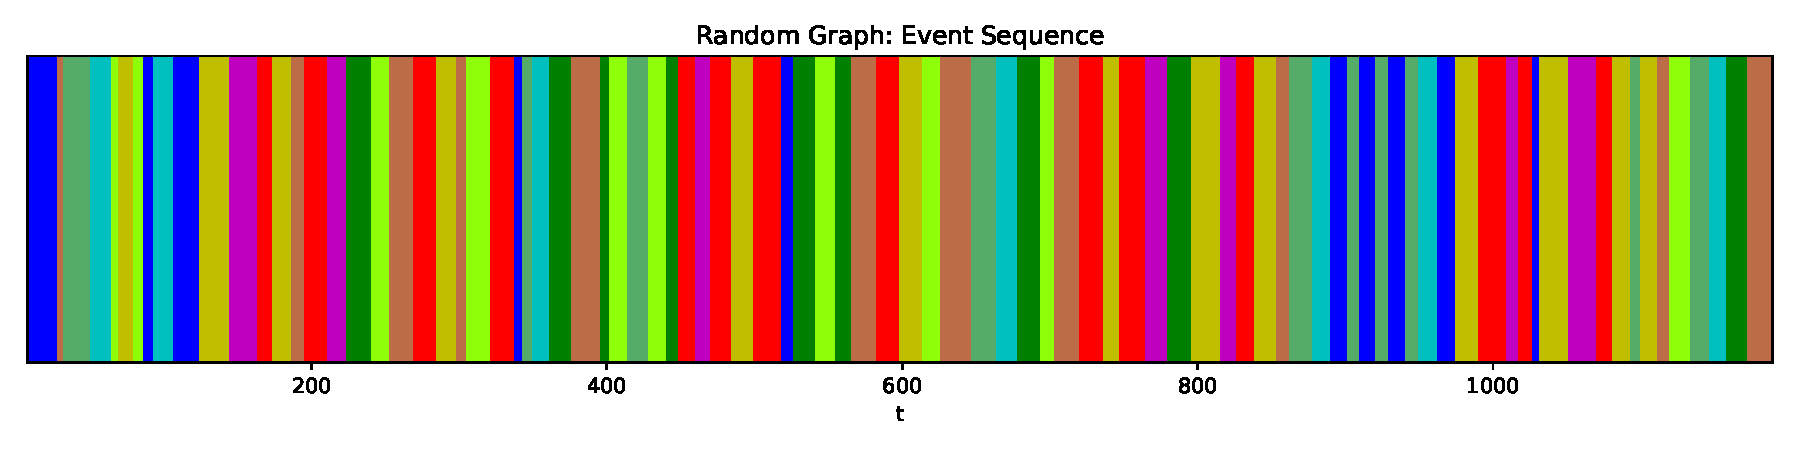
\includegraphics[width=\linewidth]{sections/010_neurips2019/paper/images/random-graph-trace.pdf}
    \caption{Trace of events for random graph. Different colors represent different classes and width of a single column represents the time that passed.}\label{fig:random-graph-trace}
\end{figure}
